\documentclass[a4paper, oneside, 12pt]{article}

%%%%%%%%%% Paquets %%%%%%%%%%

% Paquets pour le Français
\usepackage[utf8]{inputenc} % Gestion encodages
\usepackage[T1]{fontenc} % ???
\usepackage[francais]{babel} % Typographie française

\usepackage{cleveref}

% Images
\usepackage{graphicx}

% Mise en page
\usepackage[top=2.5cm, bottom=7.5cm, left=2.5cm, right=2.5cm, footskip=4.5cm]{geometry}

% Outils pour l’écriture
\usepackage{xcolor} % Utilisé pour les hiddeux \todo
\usepackage{layout} % Pour voir les commandes utiles

% Couleurs
\usepackage{color}
\definecolor{coloration_numero_ligne}{gray}{0.6}
\definecolor{coloration_reglette}{gray}{0.5}
\definecolor{coloration_fond}{rgb}{1, 1, 1}
\definecolor{coloration_commentaire}{rgb}{0, 0, 0.9}
\definecolor{coloration_mot_cle}{rgb}{0.75, 0, 0}
\definecolor{coloration_chaine}{rgb}{1, 0.2, 1}
\definecolor{coloration_type}{rgb}{0, 0.7, 0}
\definecolor{coloration_erreurs}{rgb}{0.6, 0.35, 0.8}

% Tabulations verbatim
% http://www.grappa.univ-lille3.fr/FAQ-LaTeX/6.16.html
\makeatletter
{\catcode`\^^I=\active
\gdef\verbatim{\catcode`\^^I=\active\def^^I{\hspace*{4em}}%
\@verbatim \frenchspacing\@vobeyspaces \@xverbatim}}
\makeatother

% Coloration syntaxique
\usepackage{minted}
\newminted[shellcode]{shell}{tabsize=4,xleftmargin=1cm,fontsize=\footnotesize,frame=leftline}
% On trouvera probablement difficilement mieux…
\newminted[kamcf]{ini}{tabsize=4,xleftmargin=1cm,fontsize=\footnotesize,frame=leftline}

%%%%%%%%%% Commandes supplémentaires %%%%%%%%%%%

% Marquage du travail restant
% [#1] Texte à afficher
\newcommand{\todo}[1][Il y a là encore des choses à écrire !]{\colorbox{yellow}{#1}}

%%% Gestion du sommaire
% Section non numérotée
% {#1} Nom de la section
\newcommand{\sectionSpeciale}[1]{\section*{#1}\addcontentsline{toc}{section}{#1}}
% Section non numérotée dont le titre n’est pas affiché.
% {#1} Nom de la section
\newcommand{\sectionCachee}[1]{\addcontentsline{toc}{section}{#1}}

%%% Gestion des annexes
\makeatletter
	
	\newcounter{annctr}
	
	% Définir une annexe
	% {#1} Nom de l’annexe
	\newcommand{\annexe}[1]{\stepcounter{annctr}\addcontentsline{ann}{section}{\protect\numberline {\Alph{annctr}}#1}\section*{\numberline {\Alph{annctr}}#1}}
	% Lister les annexes
	% Note : ce serait quand même bien de le faire fonctionner sans avoir besoin du makefile.
	\newcommand\listeannexes{\sectionSpeciale{Annexes}\input{annexes.tex}}
	
	% Déclaration et ouverture du fichier de stockage de la liste des annexes
	\newwrite\tf@ann
	\immediate\openout\tf@ann\jobname.ann\relax
      
\makeatother

%%%%%%%%%% Abréviations %%%%%%%%%%
% Le contenu suffit comme documentation…

\newcommand\win{Windows}
\newcommand\mac{Mac}
\newcommand\lnx{Linux}
\newcommand\lnp{Linphone}

\newcommand\my{MySQL}
\newcommand\kam{Kamailio}
\newcommand\rad{RADIUS}
\newcommand\frad{FreeRADIUS}
\newcommand\apa{Apache}
\newcommand\pma{phpMyAdmin}
\newcommand\xlite{X-Lite}
\newcommand\cph{Cisco phone \todo[(remplacer par la référence)]}
\newcommand\ata{ATA}


\begin{document}

%%% Page de garde %%%

% Pas de numéro sur cette page
\thispagestyle{empty}

% Note : logo disponibles sur http://fc.isima.fr/~brunot/files/isima/logos/
% J’avais trouvé une version vectorielle, ce serait mieux, mais je ne la trouve plus…

\includegraphics[width=6cm]{isima.png}

\vspace{0.5cm}

\begin{minipage}{4cm}
\begin{flushleft}
	Institut Supérieur d’informatique, de Modélisation et de leurs Applications
	
	\vspace{0.5cm}
	
	\small{ Campus des Cézeaux \\ 24 rue des Landais \\ BP 10125 \\ 63173 Aubière CEDEX }
\end{flushleft}
\end{minipage}

\vspace{4cm}

\begin{center}
	Rapport d’ingénieur \\
	Projet de 2{\ieme} année \\
	Filière {\em{Réseaux et télécommunications}} \\
	\Large{Facturation d’appels sur un serveur Kamailio/Radius}
\end{center}

\vspace{2cm}

\large{
\begin{tabular}{ll}
\textit{Présenté par :} & \textbf{Lucien Guimier} \\
& \textbf{Damien Teyssier}
\end{tabular}
}

\todo

\newpage
	
%%% Avant-propos %%%
\pagenumbering{roman}

\sectionSpeciale{Remerciements}

\todo
\newpage

\sectionCachee{\listfigurename}
\listoffigures
\newpage

\sectionSpeciale{Résumé}

\todo

\vspace{10cm}

\sectionSpeciale{Abstract}

\todo
\newpage

\renewcommand{\contentsname}{Table des matières}
\sectionCachee{\contentsname}
\tableofcontents
\newpage

% Sauvegarde du numéro de la page courante
\newcounter{metapage}
\setcounter{metapage}{\value{page}}
% Remise à zéro des numéros de page & changement de chiffres
\pagenumbering{arabic}

%%% Contenu %%%

\sectionSpeciale{Introduction}

La VoIP est devenue l'avenir de nos conversations téléphoniques. En effet, la téléphonie commutée (dite classique) est vouée à disparaitre dans un avenir proche. Dans le milieu des entreprises, la VoIP est aujourd'hui majoritaire même si la transition fût difficile à cause des coûts qu'elle demandait aux entreprises. Cependant, cette solution a un avantage de coût à long terme puisque qu'elle permet de faire passer toutes les communications sur le réseau de transfert de données et ainsi réduire les coûts de communication.

C'est pour cette raison que l'on nous a demandé de continuer le projet de madame Salimata \nom{Ndiaye} et monsieur Quentin \nom{Volant}. On a donc dû suivre leur protocole afin de pouvoir remonter un serveur de téléphonie en VoIP {\kam} et un serveur d'authentification {\rad}.

Nous devions ainsi réécrire une procédure d'installation de ces serveurs et, ensuite, coder une application de facturation des communications VoIP pouvant être utilisée par une entreprise.

Dans un premier temps, nous allons voir notre protocole d'installation des serveurs {\kam} et {\frad}. Nous allons ensuite expliquer les différents outils de communication que nous avons essayés d'utilisés sur notre serveur. Finalement, nous présenterons le fonctionnement de l'application de facturation.
\newpage

% Première section : organisation du projet
\section{Organisation du projet}

\subsection{Organisation temporelle}

\todo[Les fameux diagrammes de Gantt…]

\subsection{Installation des serveurs}

Nous avons passé une grande partie du temps pendant lequel nous avons travaillé sur le projet pour monter les serveurs. Durant la première phase, nous avons travaillé parallèlement sur deux machines avec des configurations légèrement différentes. Lucien travaillait sur la version disponible dans le dépôt de paquets maintenu par {\kam}, tandis que Damien travaillait sur une version compilée à partir des sources. Lorsque nous avons réalisé que les paquets proposés n’avaient pas été compilés avec une configuration permettant la communication prévue avec {\frad}, nous nous sommes concentrés sur la version directement compilée à partir des sources, comme l’avaient fait nos prédécesseurs.

Durant le temps de montage du premier serveur, notre travail s’est progressivement organisé et ce manque d’organisation initiale, conjointement avec les difficultés que nous avons rencontrées pour faire communiquer {\kam} et {\frad}, ont causé un manque de notes structurées permettant de monter efficacement le second serveur.

C’est pour cette raison que nous avons ensuite fortement séparé les tâches : Damien s’est concentré sur l’installation du second serveur, afin de disposer d’une procédure d’installation propre, et Lucien s’est occupé de la configuration des clients matériels et de l’écriture de l’interface de facturation. Cette séparation n’a pas été stricte et nous avons pu à de nombreuses occasions nous aider sur les points difficiles.

\subsection{Écriture de l’interface de facturation}

Le cahier des charges de notre projet nous imposait de travailler en PHP. Nous avons structuré notre code grâce à la syntaxe orientée objet disponible en PHP 5 et le développement a été réalisé sur plusieurs installations différentes :
\begin{itemize}
	\item notre serveur, qui dispose de la dernière version dans les paquets de la distributions que nous avons utilisée, la 5.4.36 ;
	\item le serveur web de l’ISIMA, \texttt{fc.isima.fr}, qui dispose d’une ancienne version qui n’est plus supportée mais encore appréciée pour sa stabilité, la 5.3.3 ;
	\item l’ordinateur de Lucien, qui dispose de la version 5.5.? \todo{regarder le numéro de patch}.
\end{itemize}

Afin de pouvoir travailler simultanément sur le code, nous avons utilisé le gestionnaire de versions Git, avec un dépôt commun sur Github, disponible à l’adresse
\begin{verbatim}
https://github.com/Guimier/projet2-php
\end{verbatim}

Nous nous sommes efforcés de conserver à jour une documentation de bas niveau, grâce au logiciel Doxygen, qui permet de documenter directement les classes et les méthodes dans les commentaires du code. Cette documentation est générée par la commande \texttt{doxygen} exécutée dans le répertoire racine du dépôt Git.

\newpage

% Seconde section : installation de serveurs
\section{Installation}

\subsection{Installation du système}

\todo[Trouver la version de Debian]

La première étape de notre projet consistait en l’installation de serveurs de téléphonie SIP. Nous en avons installé deux, fontionnant avec le système d’exploitation Debian. Conformément à notre cahier des charges, nous y avons installé un proxy SIP, {\kam}, attaché à un serveur d’authentification {\rad}, {\frad}.

\subsection{\kam}

\subsubsection{Installation}

Pour installer {\kam}, il nous a fallu commencer par installer les dépendances qui n’étaient pas encore présentes dans le système, disponibles dans les paquets :

\begin{itemize}
	\item{gcc} ;
	\item{bison} ;
	\item{libmysqlclient-dev} ;
	\item{libradiusclient-ng-dev} ;
	\item{mysql-server} ;
	\item{mysql-client} ;
	\item{make}.
\end{itemize}

Nous avions initialement envisagé d’utiliser ensuite les paquets Debian disponibles sur les serveurs de {\kam}, mais le paquet de base n’est pas compilé avec le support de {\rad}, rendant le paquet des bibliothèques d’authentification {\rad} inopérant.

Nous avons donc téléchargé et décompressé les sources de {\kam} pour les compiler. Nous avons choisi d’utiliser la dernière version disponible, qui était la version 4.2.2. Pour cela, nous avons utilisé les commandes :

\begin{shellcode}
wget http://www.kamailio.org/pub/kamailio/4.2.2/src/kamailio-4.2.2_src.tar.gz
tar xvf kamailio-4.2.2_src.tar.gz
\end{shellcode}

Puis nous sommes allés dans le dossier ainsi créé, pour notre part kamailio-4.2.2 et nous avons exécuté :

\begin{shellcode}
make cfg
\end{shellcode}

Cette commande construit la configuration par défaut pour la compilation, qu’il a fallu adapter à nos besoins. Conformément aux indications du rapport de l’année dernière, nous avons effectué les modifications suivantes :

\begin{itemize}
	\item{dans la liste de modules exclus du fichier \texttt{module.lst}, nous avons retiré les noms des modules concernant {\my} et {\rad}}.
\end{itemize}

Nuos avons ensuite compilé et installé {\kam} :
	
\begin{shellcode}
make all
make install
\end{shellcode}

Cette dernière commande installe {\kam} dans \texttt{/usr/local}.

\subsubsection{Configuration}

Nous avons dû ensuite configurer {\kam}. Nous sommes allés dans le dossier \texttt{/usr/local/etc/kamailio}. Il a fallu rajouter les lignes suivantes dans le fichier de configuration \texttt{kamailio.cfg} :

\#!define WITH\_MYSQL

\#!define WITH\_AUTH

\#!define WITH\_USRLOCDB

\#!define WITH\_NAT

Nous avons alors créé puis configuré la base de données. Pour la créer, il a fallu d'abord préciser quel système de base de données nous allions utiliser.
Dans notre cas, c'est mysql. C'est pourquoi il a fallu aller dans le fichier \texttt{/usr/local/etc/kamailio/kamctlrc} afin de décommenter la ligne :

DBENGINE=MYSQL

Ensuite, nous avons tapé 
\begin{shellcode}
/usr/local/sbin/kamdbctl create
\end{shellcode}
\todo

\subsection{\frad}
\subsubsection{Installation}

Nous avons choisi ensuite d'installer {\frad} à partir des paquets présents sur la machine. Pour cela, il a fallu taper la commande :

\begin{shellcode}
apt-get install freeradius
\end{shellcode}

Il fallait aussi installer les outils nécessaires au bon fonctionnement de {\frad} :

\begin{shellcode}
apt-get install freeradius-utils
\end{shellcode}

Puis, pour finir, nous avons installé un client Radius nommé Radiusclient grâce à la commande suivante :

\begin{shellcode}
apt-get install radiusclient1
\end{shellcode}

\subsubsection{Configuration}
Nous avions fini d'installer {\frad}. Il nous restait donc à le configurer. Ce serveur {\rad} peut être configuré de deux manières différentes. Soit à partir des fichiers présents dans \texttt{/etc/freeradius}, soit à partir d'une base de données. Nous avons choisi de configurer à partir des fichiers. Il a donc fallu aller vérifier si la configuration se faisait bien grâce aux fichiers. Pour cela, il a suffi d'aller vérifier dans le fichier \texttt{/etc/freeradius/sites-available/default}.

Ensuite, nous sommes allés dans le répertoire \texttt{/etc/freeradius} afin de modifier le fichier \texttt{users}. Dans ce fichier, nous avons ajouté des utilisateurs de la façon suivantes :

login Cleartext-Password:="password"

Cette ligne autorise l'utilisateur login à se connecter avec le mot de passe "password".

Nous avons pû ensuite faire le test en utilisant la commande suivante :

\begin{shellcode}
radtest login password localhost 0 testing123
\end{shellcode}

Le paramètre "testing123" est le mot de passe donné par défaut au client localhost dans le fichier \texttt{/etc/freeradius/client.conf}. Nous l'avons ensuite changé en "kamailio".


\subsubsection{Intégration de {\rad} à {\kam}}

Pour commencer, il a fallu copier les dictionnaires \texttt{/usr/local/etc/kamailio/dictionary.kamailio} et \texttt{/usr/local/etc/kamailio/dictionary.sip} dans le répertoire \texttt{/etc/radiusclient-ng}.

\begin{shellcode}
cp /usr/local/etc/kamailio/dictionary.kamailio /etc/radiusclient-ng

cp /usr/local/etc/kamailio/dictionary.sip /etc/radiusclient-ng
\end{shellcode}

Puis, nous avons inclus dans \texttt{/etc/radiusclient-ng/dictionary} les deux fichiers suivants :

\begin{itemize}
\item{\texttt{/etc/radiusclient-ng/dictionary.kamailio}}
\item{\texttt{/etc/radiusclient-ng/dictionary.sip}}
\end{itemize}

Puis il a fallu décommenter les lignes des attributs ou des valeurs Failed, Sip-Session et Call-Check dans les trois fichiers dictionary.

Nous avons ensuite dû vérifier que les deux lignes suivantes,qui donnent l'adresse du serveur {\rad}, se trouvaient bien dans le fichier \texttt{/etc/radiusclient-ng/radiusclient.conf} :

\begin{itemize}
\item{authserver localhost}
\item{acctserver localhost}
\end{itemize}

Nous avons ensuite été modifier le fichier \texttt{/etc/radiusclient-ng/servers}. Nous avons annoncé notre serveur de la façon suivante :


192.168.102.120		kamailio


Ce fichier contient l'adresse des serveurs {\rad} et leurs clefs. Ainsi nous avons choisi la clef "kamailio".

Puis ensuite il a fallu aller modifier le fichier \texttt{/etc/freeradius/clients.conf} qui définit les clients autorisés par le serveur {\frad} :

\begin{shellcode}
Client localhost
{
 ipaddress = 192.168.102.120
 secret = kamailio
}
\end{shellcode}

Nous avons dû ensuite modifier le fichier \texttt{/etc/freeradius/users}. Nous avons tout effacer et avons écrit les utilisateurs autorisés ou pas de la manière suivante :


7000@192.168.102.120 Auth-Type=Accept
7001@192.168.102.120 Auth-Type=Accept
7003@192.168.102.120 Auth-Type=Reject


Cela autorise les utilisateurs 7000 et 7001 mais rejette l'utilisateur 7002.

Ainsi nous avons deux sécurités à passer afin de pouvoir utiliser le serveur {\kam}. Il faut tout d'abord être dans la base de donnée de {\kam} puis ensuite dans le fichier users de {\frad} en tant qu'utilisateur accepté.



\newpage

% Troisième section : clients SIP
\section{Clients SIP}

Afin de tester le bon fonctionnement des serveurs et de remplir les journaux, nous avons dû utiliser des clients SIP. Nous avons principalement utilisé les clients logiciels, mais nous avons aussi essayé des clients matériels.

\subsection{\xlite}

\begin{figure}[h]
\begin{center}
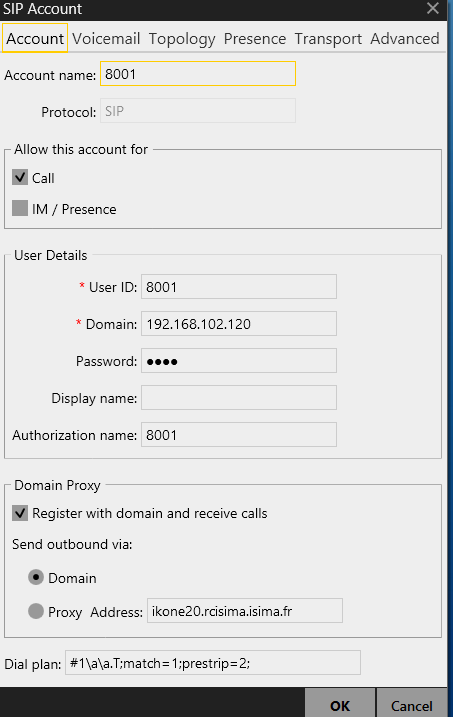
\includegraphics[width=7cm]{images/config-xlite.png}
\end{center}
\caption{Panneau de configuration de Xlite}
\label{confxlite}
\end{figure}

Suite à la rapide présentation qui nous en avait été faite en cours de téléphonie, nous avons commencé par utiliser {\xlite}. {\xlite} est un client SIP logiciel développé par la société CounterPath. Il est disponible pour {\win} et {\mac}. Le fait qu’il ne soit plus disponible pour {\lnx} nous a amenés à peu l’utiliser, afin de simplifier notre organisation. Vous pouvez, néanmoins, voir la fenêtre de configuration de Xlite à la \cref{confxlite}. 

\subsection{\lnp}

\begin{figure}[h]
\begin{center}
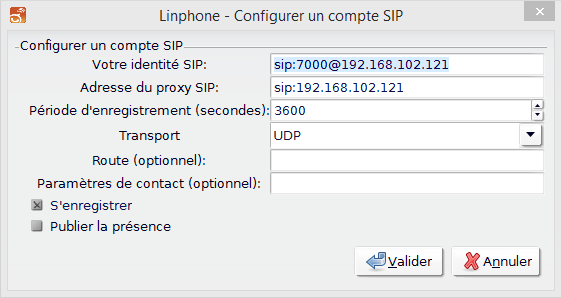
\includegraphics[width=12cm]{images/config-linphone.png}
\end{center}
\caption{Panneau de configuration de Linphone}
\label{conflinphone}
\end{figure}

Nous avons donc recherché un client logiciel disponible pour {\lnx} ; après avoir testé plusieurs logiciels non fonctionnels à cause d’erreurs de compilation, dues à des incompatibilité avec des bibliothèques trop récentes, et d’erreurs de segmentation à l’exécution, nous avons trouvé {\lnp}, qui fonctionne bien et qui a l’avantage d’être disponible dans les dépôts de la plupart des distributions {\lnx}.
Vous pouvez voir, sur la \cref{conflinphone}, la fenêtre de configuration de ce softphone. En premier lieu, vous devez configurer l'identité de votre softphone comportant son numéro et son domaine. S'ensuit alors la configuration de l'adresse IP du proxy SIP. On peut aussi configurer le protocole de la couche transport que l'on souhaite utiliser mais nous avons laissé le protocole UDP qui était par défaut.  

{\lnp} est un logiciel \textit{open source} disponible pour les principaux systèmes d’exploitation, aussi bien bureau que mobile.

\subsection{\cph}

\begin{figure}[H]
\begin{center}
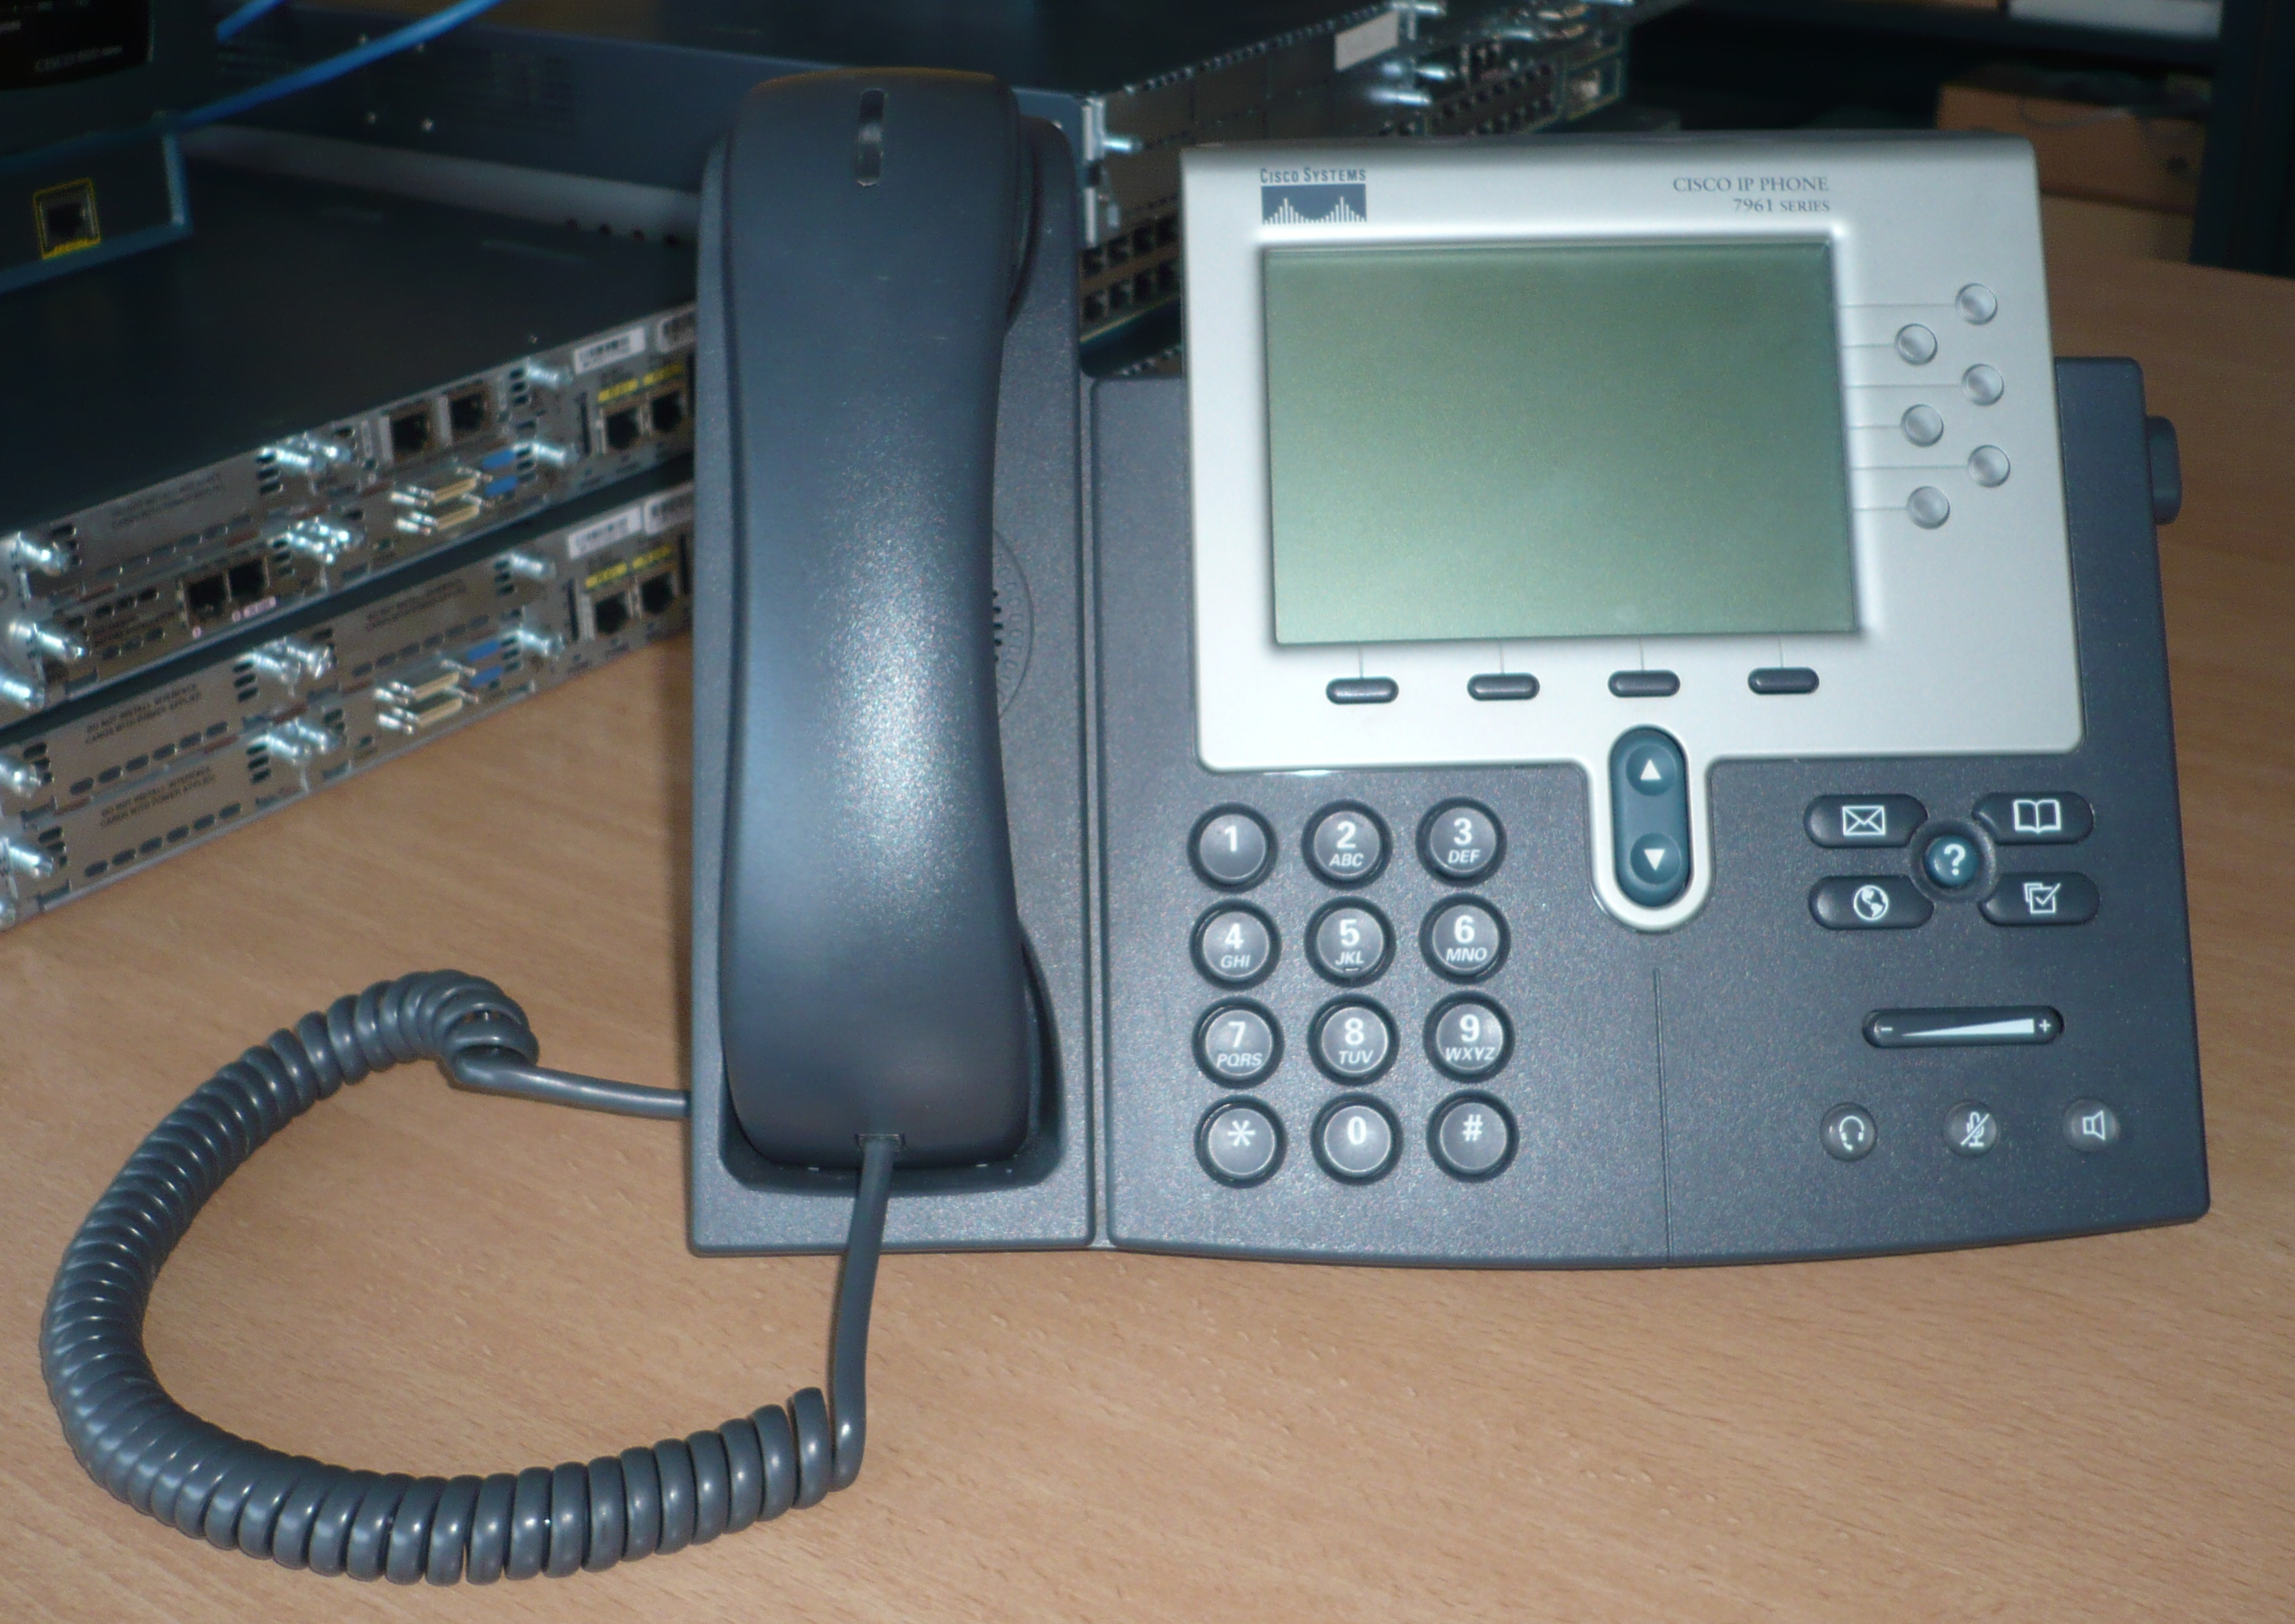
\includegraphics[width=7cm]{images/7961.jpg}
\end{center}
\caption{\cph}
\end{figure}

Le {\cph} est un téléphone fonctionnant en VoIP vendu par Cisco. Nous avons tenté d'utiliser un {\cph} dans le cadre de notre projet. Pour cela, il a fallu installer un serveur TFTP afin de permettre au téléphone de trouver sa configuration.
Nous avons néanmoins rapidement rencontré des problèmes avec cette configuration puisque la documentation semblée ne pas vouloir s'offrir à nous.
C'est pourquoi nous avons décidé d'utiliser plutôt un {\ata}.

\newpage

\subsection{\cata}

\begin{figure}[h]
\begin{center}
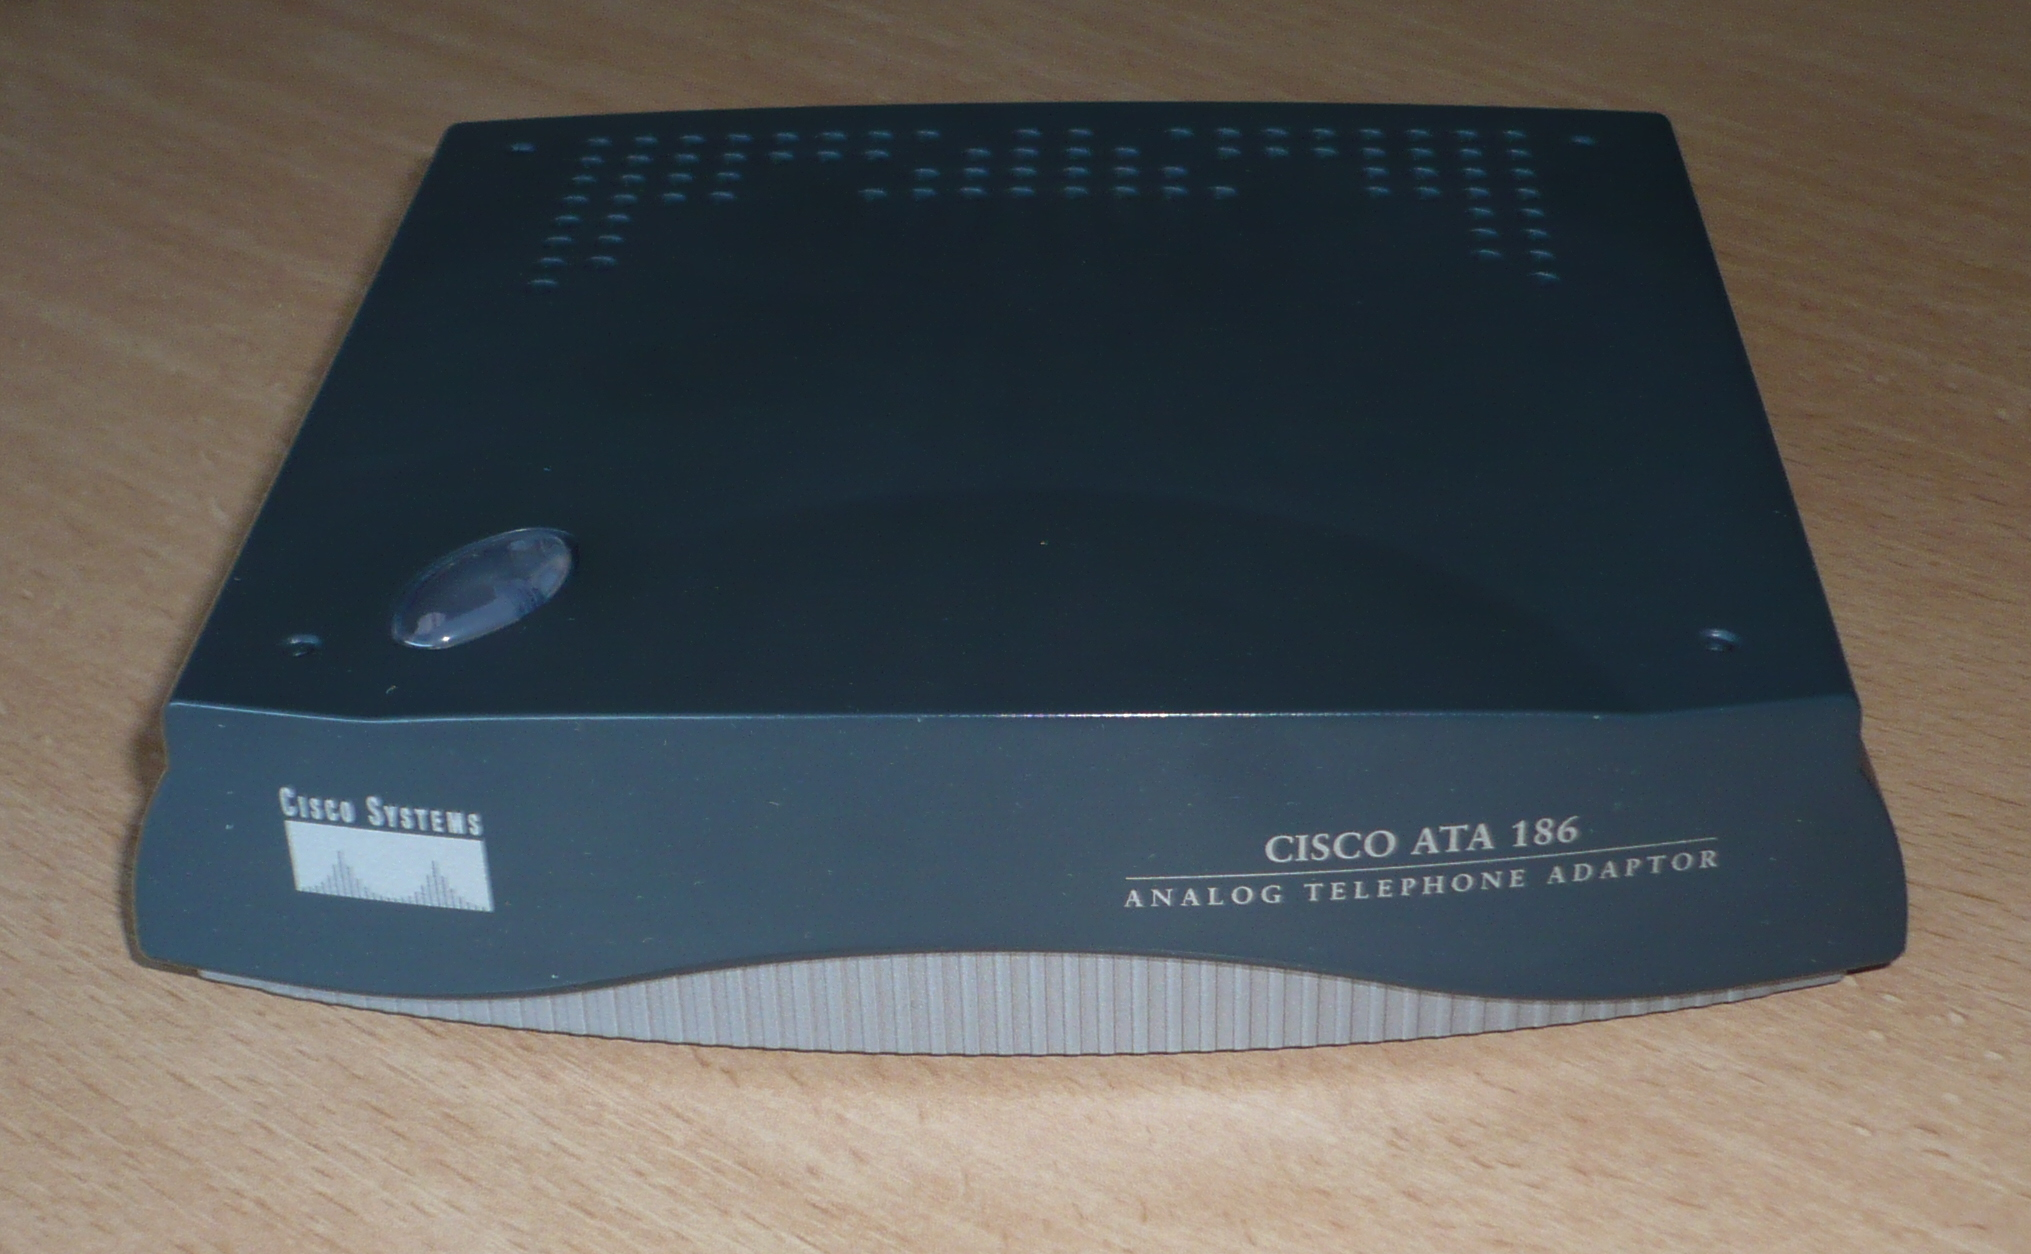
\includegraphics[width=7cm]{images/ata.jpg}
\end{center}
\caption{\ata}
\end{figure}

Un {\ata} (Analog Telephone Adaptor) est un adaptateur combiné à Ethernet permettant de faire fonctionner un téléphone analogique en VoIP. Nous en avons donc utilisé afin de pouvoir téléphoner sur notre serveur avec des téléphones analogiques. Nous ne sommes malheureusement pas parvenu à configurer l'{\ata} pour qu'il puisse lire les noms de domaine, d'où le fait que nous n'avons travaillé qu'avec les adresses IP.

\newpage

% Quatrième section : création de l’interface
\section{Création de l’interface de facturation}

\subsection{Lecture du journal créé par \frad}

\subsubsection{Accès au journal}

Le fichiers constituant le journal que crée {\frad} sont situés dans le dossier \texttt{/var/log/freeradius/radacct/127.0.0.1}. Un fichier est créé chaque jour d’activité, son nom étant de la forme \texttt{detail-aaaammjj} où \texttt{a}, \texttt{m} et \texttt{j} représentent les chiffres de l’année, le mois et le jour du mois.

Lors de l’installation, tous ces fichiers sont accessibles uniquement à \texttt{root}. Nous avons dans un premier temps modifié le groupe des répertoires pour permettre au démon HTTP d’accéder aux fichiers et nous avons configuré le dernier répertoire en mode \texttt{setgid} afin que les nouveaux fichiers héritent du bon groupe.

Cependant cette configuration n’a pas été suffisante, car {\frad} créer les fichiers avec des droits de lecture uniquement pour l’utilisateur propriétaire. Afin de nous concentrer sur le cœur du projet, nous nous sommes contentés d’une solution simple, consistant à ajouter un job dans la \texttt{crontab} donnant régulièrement les droits au démon HTTP sur les fichiers nouvellemnt créés.

Pour notre confort pendant le travail, nous avons choisi une fréquence relativement élevée, mais une fréquence nettement plus faible — le premier du mois par exemple — serait suffisante sur un serveur en production et représente un charge négligeable pour le système. Cependant il aurait pu être intéressant de configurer ce comportement directement dans {\frad} ou de l’intégrer dans un script de déplacement des fichiers (permettant leur classement et donc une meilleure lisibilité, le répertoire pouvant se remplir vite avec un fichier par jour).

\subsubsection{Format du journal}

\begin{figure}[h!]
\begin{verbatim}
Mon Jan 19 10:52:26 2015
	Acct-Status-Type = Start
	Service-Type = SIP
	Sip-Response-Code = 200
	Sip-Method = Invite
	Event-Timestamp = "Jan 19 2015 10:52:26 CET"
	Sip-From-Tag = "1514023998"
	Sip-To-Tag = "DbEJdfR"
	Acct-Session-Id = "48771904"
	Calling-Station-Id = "sip:8000@ikone20.rcisima.isima.fr"
	Called-Station-Id = "sip:8001@ikone20.rcisima.isima.fr"
	NAS-Port = 5060
	Acct-Delay-Time = 0
	NAS-IP-Address = 127.0.0.1
	Acct-Unique-Session-Id = "313763d445993202"
	Timestamp = 1421661146
\end{verbatim}
\caption{Exemple d’enregistrement dans le journal de \frad}
\label{radrecord}
\end{figure}

\todo[Rappeler ici la ligne de configuration de {\kam} qui permet l’extension.]

Ces fichiers sont constitués d’une liste d’enregistrements correspondant à des actions des utilisateurs, séparés par un double saut de ligne. Chacun de ces enregistrements commence par une date formatée, puis est constitué d’une liste de champs extensible (voir \cref{radrecord}).


Le champ \texttt{Acct-status-Type} permet de connaître le type d’action qui a provoqué la journalisation. Nous avons rencontré trois valeurs lors de nos essais :
\begin{description}
	\item[\texttt{Start}] Début d’un appel, a lieu lorsque l’appelé décroche.
	\item[\texttt{Stop}] Fin d’un appel, a lieu lorsque l’une des deux personnes communicant raccroche.
	\item[\texttt{Failed}] Appel avorté, a lieu lorsque l’appelant abandonne ou lorsque l’appelé décline l’appel.
\end{description}


\subsection{Affichage des rapports}

Dans un premier temps, nous avons vérifié le fonctionnement du système de lecture du journal grâce à un script simple exécuté en console, puis nous avons travaillé sur un système de construction de pages HTML.

\subsubsection{Architecture de l’affichage}

L’affichage est réalisé grâce à un ensemble de classes héritant de la classe abstraite \classe{Page} (un diagramme recensant ces classes est fourni en annexe), ce qui permet d’uniformiser les comportements en les intégrant à une base commune, stockée dans un fichier \texttt{template.php}.

La construction de l’interface est effectuée en deux étapes, exécutées immédiatement l’une après l’autre dans le fichier \texttt{index.php} : l’object \classe{Page} est instancié ; il stocke les paramètres du constructeur — la configuration et les paramètres de la requête — puis appelle la méthode \texttt{build}, définie par les sous-classes. Cette méthode a pour rôle la récupération des données à afficher. Dans le cas ou l’exécution de cette méthode lève une exception, la page construit un objet \classe{ExceptionPage} qui affichera l’exception.

La seconde étape est l’envoi des données à l’utilisateur, qui a lieu lors de l’appel de la méthode \texttt{display}. Celle-ci consiste en l’inclusion du fichier \texttt{template.php} ou, le cas échéant, en la délégation à la méthode \texttt{display} de l’objet \classe{ExceptionPage} créé. Le fichier \texttt{template.php}, une fois inclus, se comporte comme une partie de la méthode \texttt{build} et accède aux deux méthodes abstraite de la classe \classe{Page}, \texttt{getContent} et \texttt{getTitle}, qui retournent respectivement le contenu de la page (chaîne de caractère contenant du HTML partiel sans balise orpheline) et son titre (chaîne de caractères). Ces deux méthodes se contentent d’effectuer le formatage des données acquises précédemment et son supposées ne pas lever d’exception.

La construction de la page dans un fichier unique \texttt{template.php} et l’utilisation des méthodes statiques de la classe \classe{Page} permettent une uniformisation aisée des pages et une modification rapide.

\subsubsection{Contextes}

Pour filtrer les listes d’appels, nous avons défini la notion de contexte. Un contexte est une collection par définition de comptes sur des serveurs quelconques. Les classes représentant un contexte implémente l’interface \classe{Context}, qui définit une méthode \texttt{contains} permettant de déterminer si un compte respecte la définition reconnaissant les éléments du contexte. Cette structure ne permet pas d’extraire une liste de tous les comptes du contexte, mais a l’avantage de pouvoir représenter un contexte inconnu, par exemple un serveur distant.

Nous avons eu besoin de quatre contextes :
\begin{itemize}
	\item \classe{Account} — un compte est un contexte ne reconnaissant que lui-même, ce qui nous permet de filtrer une liste d’appels pour présenter tous les appels concernant un unique compte ;
	\item \classe{AccountGroup} — nous avons laissé la possibilité de configurer des groupes de comptes sur le serveur dont les journaux sont traités, il s’agit du seul contexte défini par ses membres, dans le fichier de configuration ;
	\item \classe{AccountDomain} — un contexte de domaine reconnaît tous les identifiants de comptes dans le domaine (sans condition de validité du compte) ;
	\item \classe{Universe} — le contexte universel permet de clore des listes de filtres ou de représenter un filtrage nul.
\end{itemize}

\subsubsection{Affichage du journal}

Pour l’affichage des journaux, nous avons créé une classe abstraite \classe{LogPage}, descendante de \classe{Page}, récupère une liste d’appels \classe{CallList} et la formate pour l’affichage. La récupération de la liste d’appels est implémentée \textit{via} une méthode \texttt{prepareLog} qui gère la sélection de la période, mais délègue le filtrage des appels aux sous-classes \textit{via} un \classe{Contexte}.

Nous avons créé trois types de pages affichant le journal : une page affichant l’intégralité des journaux du serveur, une affichant la partie des appels concernant un groupe passé dans les paramètres et une affichant la liste des appels correspondant à un compte passé dans les paramètres.

\begin{figure}
\begin{center}
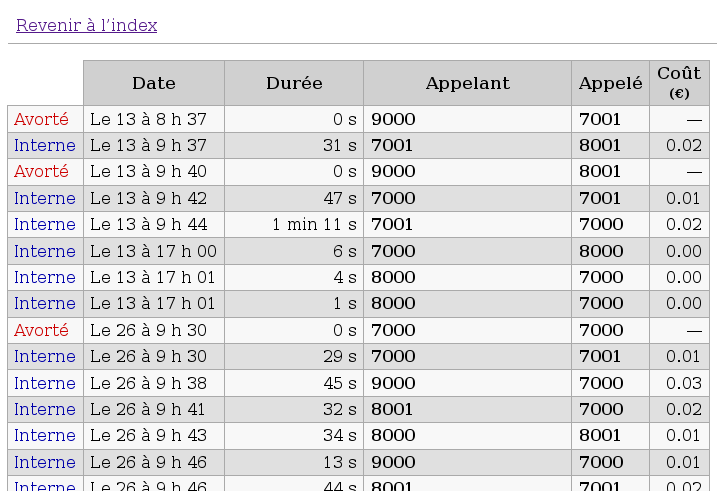
\includegraphics[width=10cm]{images/journal-global.png}
\end{center}
\label{imgjournal}
\caption{Rendu du journal global du serveur pour une série de tests}
\end{figure}

Suite à une demande de M. \nom{Laurençot}, nous avons dû ajouter à ce journal une indication des prix pour chaque appel (voir \cref{imgjournal}). Cela nous a incité à créer une classe dédiée à la gestion des prix, \classe{PriceFilters}, car les prix étaient alors gérés directement par la classe \classe{InvoicePage}.

\subsubsection{Affichage des factures}

La génération et l’affichage des factures sont gérés par une classe abstraite \classe{InvoicePage}, qui requiert la définition d’un contexte et d’une liste de filtres tarifaires par les sous-classes. Cette classe filtre tout d’abord le journal complet grâce au contexte, puis le sépare en un ensemble de listes d’appels partiels grâce à la liste de filtres tarifaires, avant de mettre en forme la facture.

Les filtres tarifaires peuvent être configurés à deux niveaux (un exemple de fichier de configuration est disponible en annexe) : pour tous les comptes du serveur, \textit{via} le tableau de configuration globale \texttt{prices}, et pour chaque groupe, \textit{via} un tableau similaire dans la définition du groupe. Ces tableaux sont des listes de couple associant un contexte à un tarif horaire. Les contextes peuvent être définis sous forme d’une chaîn de caractères : la chaîne contenant l’unique caractères \texttt{*} représente le contexte universel, les chaînes commençant par un \texttt{@} représente un domaine et les autres chaînes représentent un groupe.

Lors de la constitution de la facture, si un appel ne correspond à aucune règle du groupe concerné, les règles globales sont appliquées. Si l’appel ne correspond pas non plus à une règle globale, une exception est levée. Un serveur ouvert à n’importe quel domaine devrait donc toujours avoir une règle finale avec le contexte universel. 

\begin{figure}
\begin{center}
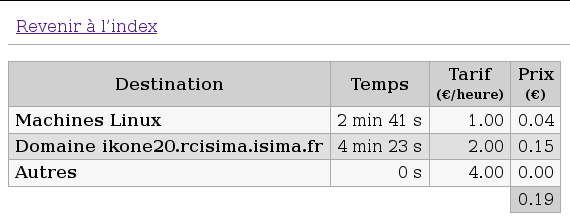
\includegraphics[width=10cm]{images/facture.png}
\end{center}
\label{imgfacture}
\caption{Rendu d’une facture}
\end{figure}




\newpage

\sectionSpeciale{Conclusion}

Il nous été demandé d'installer une solution de téléphonie SIP utilisant un proxy SIP {\kam} ainsi qu'un serveur d'authentification {\rad} {\frad}. Nous devions ensuite créer une application de facturation en utilisant les journaux de {\frad}. Durant toute la durée de notre projet, nous avons pu utiliser le matériel fourni par l'ISIMA.

Les principaux problèmes que nous avons rencontrés durant la durée de notre projet sont lié à la recherche de documentation. En effet, nous avons perdu beaucoup de temps sur ces recherches. 

Finalement, nous sommes parvenus à installer deux serveurs entre lesquels nous avons pu communiquer. Suite au montage du second serveur, nous avons réécrit une nouvelle procédure d'installation des serveurs.  
Nous avons également codé et utilisé l'application de facturation demandée.
Nous aurions cependant aimé pouvoir mieux résoudre le problème de droits des journaux d'appels de {\frad} et mieux gérer la nécessité d'utiliser des adresses IP pour l'{\ata}.


\newpage

%%% Après-propos %%%

% Changement des chiffres utilisés pour les numéros de pages
\pagenumbering{roman}
% Rétablissement du numéro de page méta
\setcounter{page}{\value{metapage}}

\sectionSpeciale{Glossaire}

\begin{description}
	\item[Crontab] ~ \newline Fichier de configuration pour les processus récurrents.
	\item[Démon]  ~ \newline Processus ou ensemble de processus s’exécutant en arrière-plan. Il s’agit du type de processus utilisé pour créer des services sur un serveur.
	\item[Proxy SIP] ~ \newline \todo
	\item[RADIUS] \textit{Remote Authentication Dial-In User Service} \newline Protocole d’authentification.
	\item[SIP] \textit{Session Initiation Protocole} \newline Protocole de contrôle des appels en VoIP. C’est le protocole responsable de l’établissement du contact et son arrêt.
	\item[VoIP] \textit{Voice over Internet Protocol} \newline Ensemble de technologies permettant le transport de la voix sur un réseau utilisant le protocole IP.
\end{description}

\newpage

\sectionSpeciale{Références}

\subsection*{Référence bibliographique}

\noindent[1] Salimata \nom{Ndiaye} et Quentin \nom{Volant}, \textit{Rapport de projet de 2\up{nde} année}, ISIMA, Aubière, 2014.

\subsection*{Webographie}

\noindent[2] \textit{Kamailio SIP Server v4.2.x (stable): Pseudo-Variables}, disponible sur : \url{http://www.kamailio.org/wiki/cookbooks/4.2.x/pseudovariables}

\noindent[3] \textit{ACC\_RADIUS Module}, disponible sur : \url{http://www.kamailio.org/docs/modules/4.2.x/modules/acc_radius.html}

\newpage

% Annexes
\listeannexes

\annexe{Diagramme de classes de la manipulation du journal}
\begin{center}
	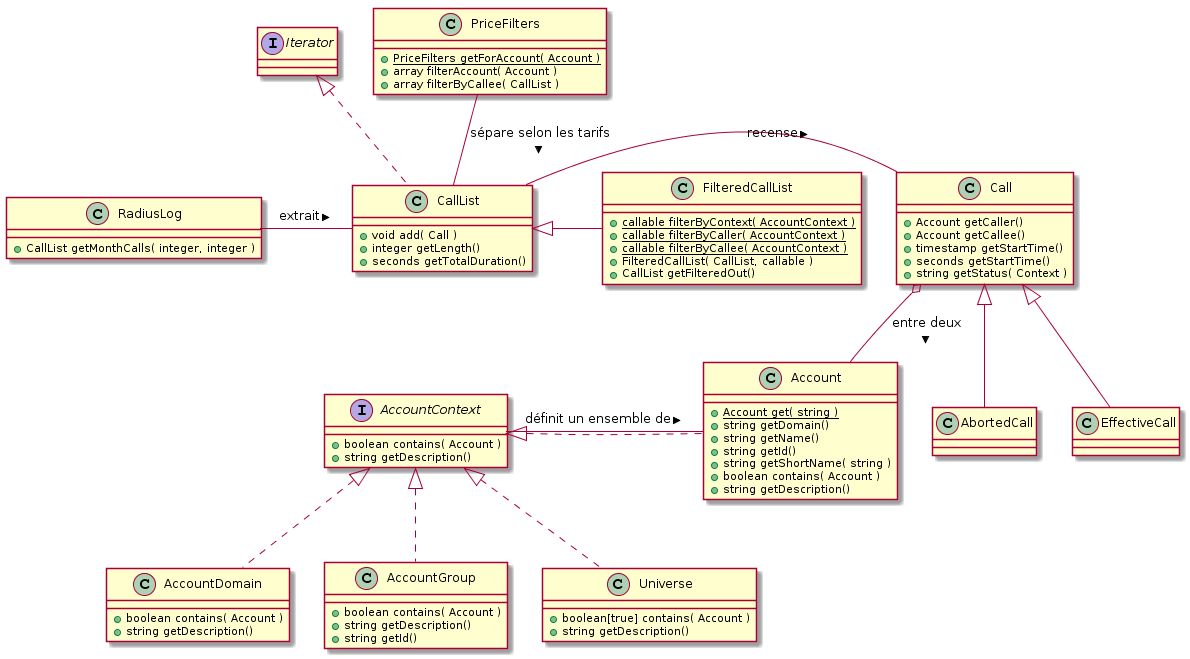
\includegraphics[angle=90, height=18cm]{uml/calls.png}
\end{center}

\annexe{Diagramme de classes de la construction de pages}
\begin{center}
	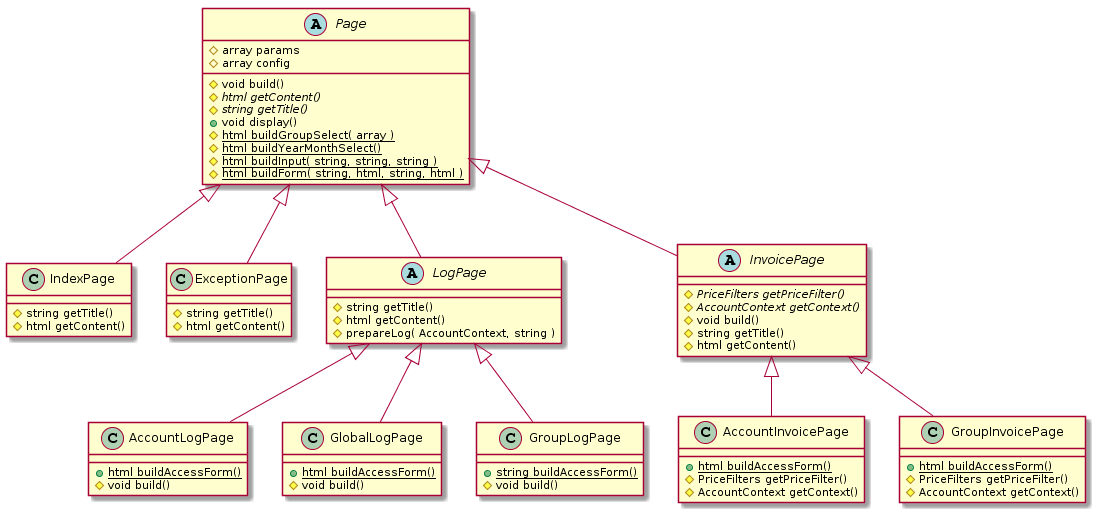
\includegraphics[angle=90, height=18cm]{uml/pages.png}
\end{center}


\end{document}
